In this section, we propose a framework for online adaptive learning for a few labeled data for both domain and target examples with deep CNN while the categories in source and target domains are different. A typical approach for domain adaption is to fine-tuning the deep CNN model with these labeled examples with low learning rate. By taking advantage of the discriminative features learned by deep CNN, this approach achieved some impressive results\cite{Chatfield14} \cite{zeiler2014visualizing}. However, fine-tuning on deep CNN requires an ample amount of labeled target data and sometimes could degrade the performance when the labeled examples are scarce\cite{hoffman2013one}. Other domain adaption methods such as Adaptive-SVM and PMT-SVM, are originally designed for learning across the similar categories and suffer from the mismatched distribution of the source and target domains, as the knowledge from source domain could be useless for target domain. In practice, people are more interested in learning the new categories in the target domain efficiently.
 As far as we know, few study has shown that there is an approach that can learn new categories with a few examples.

Chu et al. recently proposed a warm start approach for parameter selection in linear model. By iteratively updating the parameters from previous knowledge, the algorithm can search the optimal value for a specific task\cite{chuwarm}. Inspired by this, we propose a warm start adaptive learning algorithm that can adapt new categories from the target domain in an online learning scenario. Our method uses logistic regression to classify the representation obtained from deep CNN. For a new category in target domain, rather than utilizing the parameters from source domain, we introduce another affiliated binary predictor pre-trained using all the examples as the negative class and warm start the pre-trained predictor while a new category comes. This approach can be extended into an online domain adaptation scenario. Considering $M$ categories in the source domain $S$ and a new category $t$ from target domain $t$, we can train $M$ binary predictors $F=\left\{ {{f}\left( {{w_i},{b_i}} \right)} \right\}_{i = 1}^M$ for each category in $S$ and the affiliated predictor $\hat{f}=f(\hat{w},\hat{b})$ using all the examples in $\mathcal{P^-}=S$ as negative examples. The predictor $f_t$ for the new category $T$ is initialized with $\left\{\hat{w},\hat{b}\right\}$ and trained with $\mathcal{P^-}\bigcup\mathcal{P^+}$ while $\mathcal{P^+}=t$. Then we update the affiliated predictor with $\mathcal{P^-}=S\bigcup t$.
\begin{algorithm}
  \caption{Warm start online adaptation}\label{algo:ws}
  \begin{algorithmic}[1]
    \REQUIRE Source domain $S = \{ {s_i}|i = 1,..M\} $, Target domain $T = \{ {t_j}|j = 1,..N\} $, Classifier $F\leftarrow \{\emptyset\}$
    \ENSURE $F$\\
    \FORALL {$i\in M$}
         \STATE $\mathcal{P^+}\leftarrow s_i, \mathcal{P^-}\leftarrow S-s_i$\\
          Train ${{f_i}\left( {{w_i},{b_i}} \right)}$ with $\mathcal{P^+}\bigcup\mathcal{P^-}$, $F\leftarrow F\bigcup f_i$        
    \ENDFOR
    \STATE Training affiliated $\hat{f}\left( {{w_i},{b_i}} \right)$ with $\mathcal{P^-}=S$
    \WHILE {$t_j  \notin S$}
         \FORALL {$i\in M$}
             \STATE $\mathcal{P^+}\leftarrow s_i, \mathcal{P^-}\leftarrow S-s_i+t_j$ \\
              Update ${{f_i}\left( {{w_i},{b_i}} \right)}$ with $\mathcal{P^+}\bigcup\mathcal{P^-}$
        \ENDFOR
        \STATE Initialize $\hat{f_j}$ with $\left\{\hat{w},\hat{b}\right\}$ and train.
        \STATE $F\leftarrow\ F\bigcup \hat{f_j}$ 
        \STATE $D\leftarrow D\bigcup t_j, M\leftarrow M+1$ 
     \ENDWHILE
  \end{algorithmic}
\end{algorithm} 

\begin{figure*}
  \centering
  % Requires \usepackage{graphicx}
  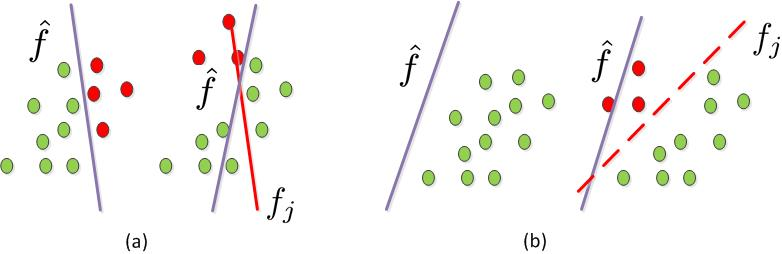
\includegraphics[scale = .6]{fig/domain.jpg}\\
  \caption{ASVM vs Ap}
\end{figure*}
